Dieses \LaTeX\ Tutorial / Template ist so aufgebaut, dass die Struktur-Informationen des zu erstellenden Dokumentes in der Haupt-Datei *.tex abgelegt ist. Alle Inhalte des Dokumentes sind in verschiedenen Verzeichnissen in weiteren Dateien enthalten.

\begin{figure}[h!]
\centering
  % 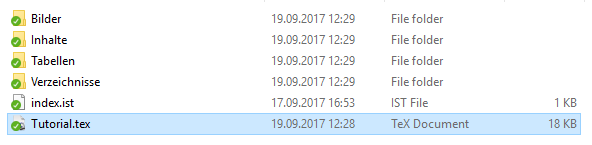
\includegraphics[width=0.75\textwidth]{./Bilder/VerzeichnisStruktur.PNG}      % Bild ohne Rahmen
  \fbox{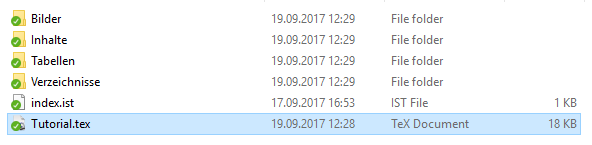
\includegraphics[width=0.75\textwidth]{./Bilder/VerzeichnisStruktur.PNG}} % Bild mit Rahmen
  \caption{Die Verzeichnis-Struktur des Dokumentes}
\end{figure}

Die Datei \menu{Tutorial.tex} ist das Kerndokument. Diese Datei ethält die Struktur (Reihenfolge der Kapitel) des Dokumentes, sowie alle benötigten Befehle für die Formatierung und für die Erstellung der verschiedenen zu generierenden Verzeichnisse (wie z.B. das Inhaltsverzeichnis, das Stichwortverzeichnis, etc.).  

Die Datei \menu{index.ist} enthält die Style-In\-for\-ma\-ti\-on\-en zum Stichwortverzeichnis. Dies wäre nicht zwingend notwendig. Da mir aber das Layout des von LaTeX automatisch erstellten Stichwortverzeichnisses nicht gefällt, habe ich dieses mit dieser Style-Datei angepasst. Dies muss in der Konfiguration von Texmaker entpsrechend angegeben werden (siehe auch \cref{fig:Konfig}: \nameref{fig:Konfig} auf Seite \pageref{fig:Konfig}).

Sämtliche (fachlichen) Inhalte des Dokumentes werden in separaten Dokumenten innerhalb der jeweiligen Verzeichnisse (Bilder, Inhalte, Tabellen, Verzeichnisse) abgelegt. Diese werden als einfache Text-Dateien mit Endung \menu{*.tex} erfasst. 

Auf den folgenden Seiten dieses Tutorials wird gezeigt, wie Text erfasst und in Absätze gegliedert wird, mit welchen Befehlen man Bilder und Grafiken einbinden kann, wie Tabellen erstellt werden, wie Querverweise innerhalb des Dokumentes erstellt werden, wie korrekt mit Abkürzungen gearbeitet wird, wie Begriffe in das Stichwortverzeichnis aufgenommen werden und wie Fussnoten sowie Literatur- / Quellenangaben erfasst  und gesetzt werden.

Dieses Tutorial / Template selbst verwendet alle im Inhaltsverzeichis aufgeführten Punkte \& Inhalte. Damit kann der Source-Text dieses Tutorials / Template \menu{Tutorial.tex} ebenfalls als Quelle für die Beantwortung vieler Fragen genommmen werden.
